%\documentclass[oneside,11pt]{book}
%\usepackage{amsmath}
%\usepackage{amsfonts}
%\usepackage{graphicx}
%\usepackage{a4wide}
%\usepackage[pdftex, plainpages=false, pdfpagelabels, pdfpagelayout=useoutlines, bookmarks, bookmarksopen=true, bookmarksnumbered=true, breaklinks=true, linktocpage, pagebackref=false, colorlinks=true, linkcolor=blue, urlcolor=blue, citecolor=blue, anchorcolor=green, hyperindex=false, hyperfigures]{hyperref}
%\usepackage{color}
%\usepackage{textcomp}
%\usepackage{amssymb}%
%\usepackage{setspace}
%\usepackage{tabularx}
%\usepackage{etex}
%\usepackage{multicol}
%\usepackage{multirow}
%\usepackage{lscape}
%\usepackage{rotating}
%\usepackage{wrapfig}
%\usepackage{float}
%\usepackage{longtable}
%\usepackage{subfigure}
%\usepackage[figurename=Fig.,labelsep=space,tableposition=top]{caption}
%\usepackage[round,colon,authoryear]{natbib}
%\usepackage{appendix}
%\usepackage{caption}
%%*********************************** To copy ligatures ********************************************************************************************* %
%%\usepackage[ansinew]{inputenc}
%\usepackage[T1]{fontenc}
%\usepackage{libertine}
%\input{glyphtounicode}
%\pdfglyphtounicode{f_f}{FB00}
%\pdfglyphtounicode{f_f_i}{FB03}
%\pdfglyphtounicode{f_f_l}{FB04}
%\pdfglyphtounicode{f_i}{FB01}
%\pdfgentounicode=1
%%**************************************************************************************************************************************************** %
%%\textwidth=445pt \hoffset=-30pt
%\usepackage{fancyhdr}   % Use fancy headers package to produce headers
%\pagestyle{fancyplain}
%\addtolength{\headwidth}{\marginparsep}
%%remember chapter and section titles
%\renewcommand{\chaptermark}[1]{\markboth{#1}{}}
%\renewcommand{\sectionmark}[1]{\markright{\thesection\ #1}}
%\lhead[\fancyplain{}{\bfseries\thepage}]{\fancyplain{}{\bfseries\rightmark}}
%\rhead[\fancyplain{}{\bfseries\leftmark}]{\fancyplain{}{\bfseries\thepage}}
%\cfoot[]{}
%\rfoot[]{}
%% Clear Header 
%% Clear Header Style on the Last Empty Odd pages
%\makeatletter
%\def\cleardoublepage{\clearpage\if@twoside \ifodd\c@page\else%
%	\hbox{}%
%	\thispagestyle{empty}%              % Empty header styles
%	\newpage%
%	\if@twocolumn\hbox{}\newpage\fi\fi\fi}
%\makeatother
%% **************************************************************************************************************************************************** %
%
%\begin{document}

%************************************************************************************************************************************************************************************************ %
\chapter{Numerical Modelling of Granular Flows}
\section{Fluid simulation using Lattice Boltzmann Method (LBM)}
The Navier-Stokes equation describes the motion of a non-turbulent Newtonian fluid. The equation is obtained by applying Newton's second law to the fluid motion, together with an assumption that the fluid stress is the sum of the viscous term, proportional to the gradient of velocity, and the pressure term. Conventional methods of Computational Fluid Dynamics (CFD) compute pertinent flow fields, such as velocity \textit{u} and pressure \textit{p}, by numerically solving Navier-Stokes equation in space \textit{x} and time \textit{t}. Alternatively, the transport equation or the Boltzmann equation, which deals with the single particle distribution function $f(x, \xi,t)$ in phase space $(x, \xi)$ and time \textit{t}, can be used to solve various problems in fluid dynamics. 

The Lattice Boltzmann Method (LBM)~\citep{Chen1998} is an alternative approach to the classical Navier-Stokes solvers for fluid flow and works on an equidistant grid of cells, called lattice cells, which interact only with their direct neighbours. In the Lattice Boltzmann Method, the discretisation of continuum equations is based on microscopic models and mesoscopic continuum theories~\citep{Chen1998}. The Lattice Boltzmann Method is a special discretising scheme of the Boltzmann equation where the particle distribution functions (mass fractions) collide and propagate on a regular grid~\citep{Zhou2012}. The important aspect, however is the \textit{discretization of the velocity}, which means that the particle velocities are restricted to a predefined set of orientations.

The theoretical premises of the LBE method are that (1) hydrodynamics is insensitive to the details of microscopic physics, and (2) hydrodynamics can be preserved so long as the conservation laws and associated symmetries are respected in the microscopic and mesoscopic level. Therefore, the computational advantages of the LBE method are achieved by drastically reducing the particle velocity space $\xi$ to only a very few discrete points without seriously degrading hydrodynamics~\citep{Mei2000}. This is possible because the LBM rigorously preserves the hydrodynamic moments of the distribution function, such as mass density and momentum fluxes, and the necessary symmetries~\citep{He1997a,He1997b}. The process of averaging the density and the momentum over some regions of the space, i.e. coarse graining, produces some useful fluid simulation. The LB method has evolved as a comprehensive fluid solver and its theoretical aspects link well with the conventional central finite difference scheme~\citep{cook2004}.


\subsection{Formulation}
The Lattice Boltzmann Method is a `micro-particle' based numerical time-stepping procedure for the solution of incompressible fluid flows. Consider a 2D incompressible fluid flow with density $\rho$ and kinematic viscosity \textit{v}, in a rectangular domain \textit{\textbf{D}}. The fluid domain is divided into a rectangular grid or lattice, with the same spacing \textit{`h'} in both the \textit{x-} and the \textit{y-}directions, as shown in Figure~\ref{fig:D2Q9}. These lattices are usually classified in the literature using the $\textit{D}\alpha\textit{Q}\beta$-notation, where $\alpha$ is an integer number denoting the space dimensionality and $\beta$ is the number of discrete velocities (but including the possibility of having particle at rest) within the momentum discretisation. The most common lattices are the $\textit{D2Q9}$ and the $\textit{D3Q19}$-models, see ~\citet{he1997}. The present study focuses on two-dimensional problems, hence the $\textit{D2Q9}$ momentum discretisation is adopted.

The Lattice Boltzmann Method discretises the Boltzmann equation in space, to a finite number of possible particle spatial positions and microscopic momenta, and time. Particle positions are confined to the nodes of the lattice. The fluid particles at each node are allowed to move to their eight intermediate neighbours with eight different velocities $\textit{e}_{\textit{i}} (\textit{i}=1,\dots,8)$. A particle can remain at the node, which is equivalent to moving with zero velocity $\textit{e}_{\textit{o}}$. The particle mass is uniform, hence these microscopic velocities and momentum are always effectively equivalent~\citep{han2007}.

\begin{figure}[htpb]
\centering
\includegraphics[width=0.8\textwidth]{Chapter3/figures/lbm/D2Q9.pdf}
\caption[The Lattice Boltzmann discretisation and D2Q9 scheme]{The Lattice Boltzmann discretisation and D2Q9 scheme: (a) a standard LB lattice and histogram views of the discrete single particle distribution function/direction-specific densities $f_i$; (b) D2Q9 model}
\label{fig:D2Q9}
\end{figure}

Referring to the numbering system shown in Figure~\ref{fig:D2Q9}, these nine discrete velocity vectors are defined as:
\begin{align} 
\begin{cases}
\textit{e}_{\textit{o}}=(0,0)\\
\textit{e}_{\textit{1}}=\textit{C}(1,0); \textit{e}_{\textit{2}}=\textit{C}(0,1); \textit{e}_{\textit{3}}=\textit{C}(-1,0); \textit{e}_{\textit{4}}=\textit{C}(0,-1); \\
\textit{e}_{\textit{5}}=\textit{C}(1,1); \textit{e}_{\textit{6}}=\textit{C}(-1,1); \textit{e}_{\textit{7}}=\textit{C}(-1,-1); \textit{e}_{\textit{8}}=\textit{C}(1,-1); \\ 
\end{cases}
\end{align}
in which \textit{C} is the lattice speed, which is defined as:
\begin{align}
\textit{C}=\textit{h}/\Delta t
\end{align}
where $\Delta \textit{t}$ is the discrete time step. The primary variables in the Lattice Boltzmann formulation are called the \textit{fluid density distribution functions}, $\textit{f}_{\textit{i}}$, each relating the portable amount of fluid particles moving with the velocity $\textit{e}_{\textit{i}}$ along the $\textit{i}^{\textit{th}}$ direction at each node. The macroscopic variables are defined as functions of the particle distribution functions (see figure~\ref{fig:D2Q9}), according to:
\begin{align} 
 \nonumber
& \rho=\sum\limits_{\textit{i}=0}^{\beta - 1}{\textit{f}_{\textit{i}}} \qquad \mbox{(macroscopic fluid density)} \\ 
 \nonumber
& \qquad \mbox{and} \\ 
& \overrightarrow{\textit{u}}=\frac{1}{\rho} \sum\limits_{\textit{i}=0}^{\beta -1}{\textit{f}_{\textit{i}}\overrightarrow{\textit{e}_{\textit{i}}}} \quad \mbox{(macroscopic velocity)}
\label{eq:lbm_macroscopic}
\end{align} 
where $\textit{i} \in [0, \beta -1]$ is an index spanning the discretized momentum space. There are nine fluid density distribution functions, $\textit{f}_{\textit{i}}(\textit{i}=0,\dots,8)$, associated with each node in the \textit{D2Q9} model. The evolution of the density distribution function at each time step for every lattice point is governed by:
\begin{align} 
\label{eq:stream}
\textit{f}_{\textit{i}}(\mathbf{x}+\mathbf{e}_{\textit{i}} \Delta t, t + \Delta t) = \textit{f}_{\textit{i}}(\mathbf{x},t) - \frac{1}{\tau} [\textit{f}_{\textit{i}}(\mathbf{x},t) -\textit{f}_{\textit{i}}^{\textit{eq}}(\mathbf{x},t)] \quad (\textit{i}=0,\dots,8)
\end{align}
where for any grid node $\mathbf{x},\mathbf{x}+\mathbf{e}_{\textit{i}} \Delta t$ is its nearest node along the direction $\textit{i}$. $\tau$ is a non-dimensional relaxation time parameter, which is related to the fluid viscosity; and $\textit{f}_{\textit{i}}^{\textit{eq}}$ is termed as the equilibrium distribution function, and is defined as:
\begin{align}
\begin{cases}
\textit{f}_{\textit{0}}^{\textit{eq}}=\textit{w}_{\textit{0}} \rho (1 - \frac{3}{2\textit{C}^{\textit{2}}}\mathbf{v}.\mathbf{v}) \\ 
\vspace*{2mm}
\textit{f}_{\textit{i}}^{\textit{eq}}=\textit{w}_{\textit{i}} \rho (1 + \frac{3}{\textit{C}^{\textit{2}}}\mathbf{e}_{\textit{i}}.\mathbf{v} \frac{9}{2\textit{C}^{\textit{2}}} (\mathbf{e}_{\textit{i}}.\mathbf{v})^{\textit{2}}-\frac{3}{2 \textit{C}^{\textit{2}}}\mathbf{v}.\mathbf{v}) \quad (\textit{i}=0,\dots,8)
\end{cases}
\end{align}
in which, $\textit{w}_{\textit{i}}$ represents the fixed weighting values:
\begin{align}
\textit{w}_{\textit{0}} = \frac{4}{9}; \quad \textit{w}_{\textit{1,2,3,4}}= \frac{1}{9}; \quad \textit{w}_{\textit{5,6,7,8}}= \frac{1}{36}
\end{align}
In addition, the right-hand side of Eq.~\ref{eq:stream} is often denoted by $\textit{f}_{\textit{i}}(\mathbf{x}, \textit{t}_{+})$ and termed the post collision distribution. The LB equation \ref{eq:stream} ensures conservation of total mass and total momentum of the fluid particles at each lattice node. It essentially consists of two phases: \textit{collision} and \textit{streaming}. The collision phase computed in the right-hand side of Eq.~\ref{eq:stream}, involves only those variables which are associated with each node \textbf{x}, and therefore is a local operation. The streaming phase then explicitly propagate the updated distribution functions at each node to its neighbours $\mathbf{x}+\mathbf{\textit{e}}_{\textit{i}} \Delta t$, where no computations are required and only data exchange between neighbouring nodes are necessary. These features, together with the explicit time-stepping nature and the use of a regular grid, make LB computationally efficient, simple to implement and natural to parallelism~\citep{han2007}. The streaming step involves the translation of the distribution functions to their neighbouring sites according to the respective discrete velocity directions, as illustrated in Figure~\ref{fig:stream} in the \textit{D2Q9} model. 
\clearpage
\begin{figure}[h]
\centering
\includegraphics{Chapter3/figures/lbm/stream.pdf}
\caption[Illustration of the streaming process on a \textit{D2Q9} lattice]{Illustration of the streaming process on a \textit{D2Q9} lattice. The magnitude of the distribution functions remains unchanged, but they move to a neighbouring node according to their direction.}
\label{fig:stream}
\end{figure}
The collision step, (illustrated in Figure~\ref{fig:collision}) consists of re-distribution of the distribution functions to the local discretized Maxwellian equilibrium distribution functions, but in such a way that local mass and momentum are invariants. In incompressible flows, the energy conservation is equivalent to momentum conservation~\citep{he1997}.
\begin{figure}[htbp]
\centering
\includegraphics{Chapter3/figures/lbm/collision.pdf}
\caption[Illustration of the collision process on a \textit{D2Q9} lattice]{Illustration of the collision process on a \textit{D2Q9} lattice. The local density $\rho$ and velocity $\mathbf{v}$ are conserved, but the distribution functions change according to the relaxation to local Maxwellian rule}
\label{fig:collision}
\end{figure} 

The standard macroscopic fluid variables, density $\rho$ and velocity $\mathbf{\textit{ v}}$, can be recovered from the distribution functions as:
\begin{align}
\rho = \sum\limits_{\textit{i}=0}^{8}{\textit{f}_{\textit{i}}}\mbox{ }; \qquad \rho \mathbf{v} = \sum\limits_{\textit{i}=0}^{8}{\textit{f}_{\textit{i}}\mathbf{\textit{e}}_{\textit{i}}}
\end{align}
The fluid pressure field \textit{p} is determined by the following equation of state:
\begin{align}
\textit{p}=\textit{C}_{\textit{s}}^{2} \rho
\end{align}
where $\textit{C}_{\textit{s}}$ is termed the fluid speed of sound and is related to the lattice speed \textit{C} by
\begin{align}
\textit{C}_{s}=\textit{C}/\sqrt{3}
\end{align}
The kinematic viscosity of the fluid \textbf{\textit{v}} is implicitly determined by the model parameters \textit{h}, $\Delta \textit{t}$ and $\tau$ as:
\begin{align}
\textit{v}=\frac{1}{3}(\tau - \frac{1}{2})\frac{\textit{h}^{2}}{\Delta \textit{t}} = \frac{1}{3}(\tau - \frac{1}{2})\textit{Ch}
\end{align}
which indicates that these three parameters are related to each other and have to be appropriately selected to represent the correct fluid viscosity. An additional constraint to the parameter selection is the lattice speed \textit{C}, which must be sufficiently large in comparison with the maximum fluid velocity $\textit{v}_{\textit{max}}$ in the simulation, to ensure accuracy of the solution. This is measured by the `computational' Mach number, $\textit{M}_{\textit{a}}$, defined by
\begin{align}
\textit{M}_{\textit{a}}=\frac{\textit{v}_{\textit{max}}}{\textit{C}}
\end{align}
Theoretically, the Mach number is required to be $\textit{M}_{\textit{a}}<< 1$. In practice, $\textit{M}_{\textit{a}}$ should be, at least smaller than 0.1~\citep{he1997}. From a computational point of view, it is more convenient to choose \textit{h} and $\tau$ as two independent parameters and $\Delta \textit{t}$ as the derived parameter, using the following equation.
\begin{align}
\Delta \textit{t} = (\tau - \frac{1}{2}) \frac{h^{2}}{3\textit{v}}
\end{align}
It can be observed that $\tau$ has to be $\tau > 1/2$ \citep{he1997}. Since there is no a priori estimation available to determine appropriate values of \textit{h} and $\tau$ for a fluid flow problem with given fluid viscosity $\textit{v}$, a \textit{trial and error} approach is employed to obtain results satisfying the requirement of smaller \textit{Mach Number}. This is similar to the choice of an appropriate Finite Element mesh size, without automatic adaptive mesh techniques. 
%************************************************************************************************************************************************************************************************ %
\subsection{Boundary conditions}
Boundary conditions (BC) form an important part of any numerical solutions. In many cases, the boundary conditions can strongly influence the accuracy of the algorithm. The velocity and pressure are not primary variables in the Lattice Boltzmann method, hence the standard pressure, velocity, and mixed boundary conditions cannot be imposed directly. Hence, alternative conditions in terms of the distribution functions are adopted to describe the boundary conditions. Various boundary conditions used in the present study are discussed below.
\subsubsection*{Periodic boundary condition}
The simplest type of boundary condition is the periodic boundary. In this case, the domain is folded along the direction of the periodic boundary pair. For boundary nodes, the neighbouring nodes are on the opposite boundary, using the normal referencing of neighbours (see Figure~\ref{fig:D2Q9}a). From the perspective of submarine landslide modelling, the periodic boundary conditions are useful for preliminary analysis, as they imply higher degree of symmetry of the fluid domain. Further information on the periodic boundary condition can be found in~\citet{aidun1998}.
\subsubsection*{No-slip boundary condition} \label{bounce}
The most commonly adopted BC in the Lattice Boltzmann approach is the no-slip BC, especially the simple bounce-back rule, which is quite elegant and surprisingly accurate. The basic idea is that the incoming distribution functions at a wall node are reflected back to the original fluid nodes, but with the direction rotated by $\pi$ radians. The bounce-back boundary condition is one of benefits of the Lattice Boltzmann method, as it is trivial to implement and it allows one to effortlessly introduce obstacles into the fluid domain. However, the boundary conditions have been proven to be only first-order accurate in time and space~\citep{pan2006}. A straightforward improvement is to consider the wall-fluid interface to be situated halfway between the wall and fluid lattice nodes~\citep{ziegler1993}. It involves, defining the \textit{solid} nodes as those lying within the stationary wall regions, and the\textit{fluid} nodes otherwise. Then if \textit{i} is the direction between a fluid node $\textit{n}_{1}$ and $\textit{n}_{2}$ to be reflected back along the direction they came from, i.e.
\begin{align}
\textit{f}_{-\textit{i}}(\mathbf{x}, \textit{t}+\Delta \textit{t}) = \textit{f}_{\textit{i}}(\mathbf{x}, \textit{t}_{+})
\end{align}
where $-\textit{i}$ denotes the opposite direction of \textit{i}. The bounce back rule is illustrated in Figure~\ref{fig:bounce}. This simple rule ensures that no tangential velocity exists along the fluid-wall interface, thereby a non-slip condition is imposed, and can be extended to any shapes or objects in a fluid flow. The slip boundary conditions have similar treatment to the non-slip condition, except that the distribution functions are reflected in the boundary instead of bounce-back~\citep{succi2001}.
\begin{figure}[htbp]
\centering
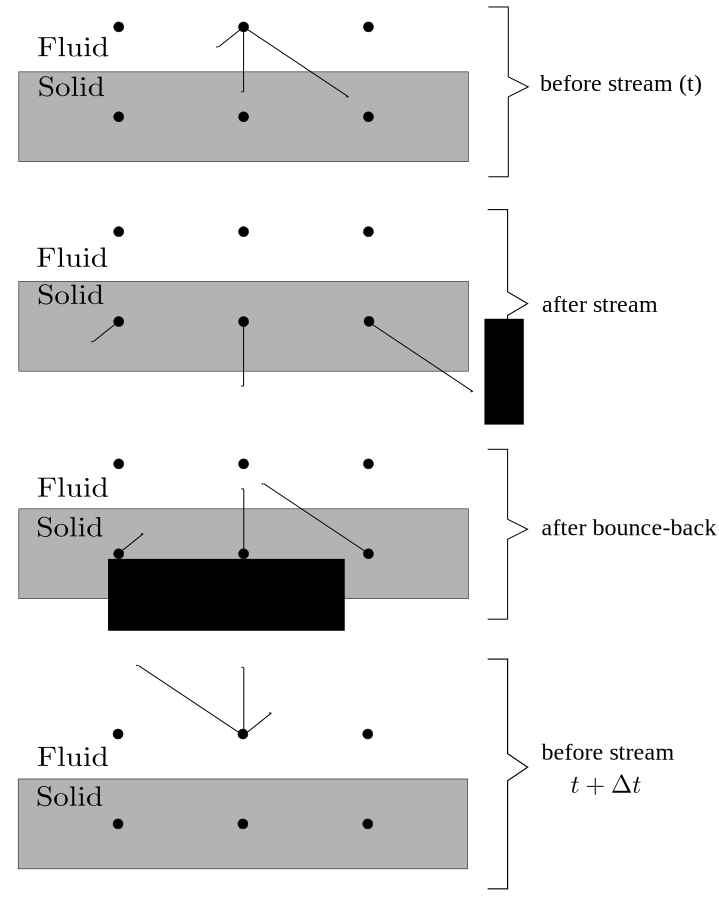
\includegraphics[scale=0.6]{Chapter3/figures/lbm/bounce.pdf}
\caption[Half-way bounce back algorithm for the \textit{D2Q9} model ]{Half-way bounce back algorithm for the \textit{D2Q9} model adopted after \citet{sukop2006}}
\label{fig:bounce}
\end{figure}

\subsubsection*{Pressure and velocity boundary condition}
The pressure (Drichlet)boundary condition can be imposed in Lattice Boltzmann by specifying a fluid density at the pressure boundary~\citep{Zou1997}. To impose a pressure boundary along the y-direction (inlet, left side boundary in Figure~\ref{fig:LBM_Poiseuille}), a density $\rho = \rho_{in}$ is specified from which velocity is computed. Assuming the vertical component of the velocity on the boundary is zero, $u_y=0$. After streaming, $f_2, f_3, f_4, f_6, f_7$ are known, $u_x$ and $f_1, f_5, f_8$ are to be determined from Eq.~\ref{eq:lbm_macroscopic} as following:
\begin{align}
f_1+f5+f_8 & =  \rho_{in} - (f_0+f_2+f_3+f_4+f_6+f_7) \label{eq:pressure1}\\
f_1+f5+f_8 & =  \rho_{in}u_x + (f_3+f_6+f_7) \label{eq:pressure2} \\
f_5 - f_8  & =  f_2 - f_4 +f_6 -f_7
\end{align}
\flushleft Consistency of Eqs.(~\ref{eq:pressure1},~\ref{eq:pressure2}) gives
\begin{align}
u_x = 1 - \frac{[f_0+f_2+f_4+2*(f_3+f_6+f_7)]}{\rho_{in}}
\end{align}
Using bounce-back rule for the non-equilibrium part of the particle distribution normal to the inlet to find $f_1 -f_1^(eq) = f_3 -f_3^(eq)$. With $f_1$ known, $f_5,f_8$ are obtained as:
\begin{align}
f_1 & = f_3 + \frac{2}{3} \rho_{in}u_x, \nonumber \\ 
f_5 & = f_7 - \frac{1}{2}(f_2 - f_4) + \frac{1}{6}\rho_{in}u_x,\nonumber \\ 
f_8 & = f_6 + \frac{1}{2}(f_2 - f_4) + \frac{1}{6}\rho_{in}u_x
\end{align}
The corner node at inlet needs some special treatment. Considering the bottom node at inlet as example, after streaming, $f_3, f_4, f_7$ are known; $\rho$ is define, and $u_x = u_y = 0$. The particle distribution functions $f_1, f_2, f_5, f_6, f_8$ are to be determined. The bounce-back rule for the non-equilibrium part of the particle distribution normal to the inlet and the boundary is used to find:
\begin{align}
f_1 = f_3 + (f_1^{eq}-f_3^{eq}) = f_3;\mbox{ }f_2= f_4 + (f_1^{eq}-f_3^{eq}) = f_4; 
\end{align}
\flushleft Using these we find: 
\begin{align}
f_5 = f_7; \mbox{  }f6 = f_8 = \frac{1}{2}[\rho_{in} - (f_1 + f_2 + f_3 + f_4 + f_5 + f_6 + f_7 + f_8)]
\end{align}
Similar procedure can be applied to top inlet node and outlet nodes. Von Neumann boundary conditions constrain the flux at the boundaries. A velocity vector $u=\left[ u_0\mbox{ }v_0 \right]^T$ is specified from which density/pressure is computed based on the domain. The velocity boundary condition can be specified in a similar way~\citep{Zou1997}. The pressure and velocity boundary conditions contribute additional equation(s) to determine the unknown distribution functions. In the velocity boundary, the equation is sufficient to determine the unknown distribution functions in \textit{D2Q9} model, however the pressure boundary conditions require additional constitutive laws to determine the unknown distribution functions. 
%************************************************************************************************************************************************************************************************ %

\section{Validation of Lattice Boltzmann Method}
The Lattice Boltzmann method implemented in the present study is validated by comparing the LBM simulation of laminar flow  through a circular pipe with the closed form solution. In the present study, water ($\rho=1000 kg/m^{3}$) is simulated to flow through a circular pipe of diameter `D' = 0.04 m and simulation length, `L' = 0.1 m. Periodic boundary conditions are applied at either end of the pipe, which simulates the condition of a continuous flow of fluid in a closed circular pipe. The parameters adopted in the LBM simulation is summarized in Table~\ref{t:lbm}. Sufficient time is allowed for the flow to travel beyond the required development length so as to develop in to a fully laminar flow~\citet{durst2005}. The development length required for a flow to be fully laminar is:
\begin{align}
X_{D}/D=[(0.619)^{1.6}+(0.0567 R_{e})^{1.6}]^{1/1.6}
\end{align}
where $X_{D}$ is the development length and $R_{e}$ is the Reynold's number. The velocity profile of water in the simulated segment at the end of the simulation is presented in Figure~\ref{fig:vel}. Figure~\ref{fig:LBM} shows the horizontal velocity profile obtained at L/2 after 50,000 time steps. The maximum horizontal velocity of 0.037863 m/s is observed in the middle of the pipe. The velocity profile obtained (Figure~\ref{fig:vel}), is compared with the closed-form based on the Haygen-Poiseuille's flow equation for no-slip boundary condition~\citep{willis2008}:
\begin{align}
\textit{v}_{\textit{x}}=\frac{\Delta P}{2 \mu L} [\frac{D^{2}}{4}-y^{2}]
\end{align}
where $v_{x}$ is the horizontal velocity (m/s); $\Delta P$ is the pressure gradient, $\mu$ dynamic viscosity of the fluid, 
 \begin{table}
\caption{LBM parameters used in simulating laminar flow through a circular pipe}
\label{t:lbm}
\centering
\begin{tabular}{|l|c|}
\hline
\textbf{Parameter} & \textbf{Value} \\ \hline \hline
Fluid & Water \\ \hline
Density $\rho$ & 1000 $kg/m^{3}$ \\ \hline
Relaxation parameter $\tau$ & 0.51 \\ \hline
Kinematic viscosity  & $ 1 \times 10^{-6} \mbox{ }m^{2}/s$ \\ \hline
Dynamic viscosity & $ 1.002 \times 10^{-3} \mbox{ }Ns/m^{2} $ \\ \hline 
Acceleration & $1 \times 10^{-6} \mbox{ m/s}$ \\ \hline
Maximum number of iterations & 50,000 \\ \hline 
Type of flow & laminar \\ \hline
Diameter of pipe `D' & 0.04 m \\ \hline
Length of the pipe `L' & 0.1 m \\ \hline
Boundary condition & Periodic boundary \\ \hline \hline
Maximum horizontal velocity at L/2 & 0.037863\mbox{ m/s} \\ \hline
Theoretical maximum horizontal velocity (Poiseuille's flow) & 0.0379\mbox{ m/s} \\ \hline
Error in predicting horizontal velocity & 0.009 \% \\ \hline
\end{tabular}
\end{table}
The horizontal velocity profile estimated at `L/2' based on the closed form solution is also plotted in Figure~\ref{fig:vel}. It can be observed from the figure that the Lattice Boltzmann method predicts the laminar flow behaviour, however the maximum horizontal velocity is underestimated by 0.009 \% in comparison to the closed form solution. To validate the Lattice Boltzmann code developed in the present study, the results of the laminar flow through a pipe is compared with those obtained from the Computational Fluid Dynamics (CFD) simulations performed using \textit{ANSYS FLUENT}. The CFD analysis involves solving problems associated with fluid flows using numerical approximations to solve Navier-Stokes equations, which defines any single-phase flow. The Finite Volume Method (FVM) is a common approach used in the CFD codes, like FLUENT. It involves solving the governing equation over the discretized control volume. This guarantees the conservation of fluxes over a particular control volume. The finite volume equations yield governing equations of the form:
\begin{align}
\frac{\partial}{\partial t} \int\int\int  Q d\mathbf{V} + \int\int \textit{F} d\mathbf{A} = 0
\end{align}
where \textit{Q} is the vector of conserved variables, \textit{F} is the vector of fluxes in the Navier-Stokes equation, \textit{V} is the volume of control volume element, and \textit{A} is the surface area of the control volume element. A 2D rectangular plane of length 1m and height 0.04m is discretized into 400 cells of size $1 \time 10^{-2} $ m (see Figure~\ref{fig:mesh}). A constant velocity is applied at the inlet. Water ($\rho = 998.2\mbox{ }kg/m^{3},\mbox{ } viscosity`\eta'=1 \times 10^{-3}\mbox{ } Ns/m^{2} $) is allowed to flow through the pipe and it develops into a fully laminar flow. The Least-Squares cell based approach was adopted to solve the gradient, and 100 iteration steps were carried out until the solution converges. The velocity contour profile obtained from the CFD analysis is presented in Figure~\ref{fig:cont}. The velocity profile at the cross-section `L/4' is plotted in Figure~\ref{fig:LBM}. The velocity profile matches the analytical Poiseuille's solution and the LBM simulation of laminar flow. Having validated the CFD analysis against Poiseuille's equation, the CFD analysis can now be used to validate the LBM simulation of fluid flow around a rectangular obstacle, to study the capability of the LBM technique to simulate vortex effects in fluid flows around obstacles.

The efficiency of Lattice Boltzmann method to include solid walls/particles is evaluated by placing a solid wall of Length `D/2' at length `L/4' in the pipe. The velocity profile obtained after 50,000 iterations is presented in Figure~\ref{fig:Obstacle}. The formation of eddies at the corners of the wall along the flow direction is captured by the LB method. The horizontal velocity profile obtained at `L/4' is presented in Figure~\ref{fig:LBM}. The occurrence of vortex effect in the flow around the edges of the obstacle can be visualized in Figure~\ref{fig:Obstacle}. The velocity profile obtained from the LBM simulation of the fluid flow around a rectangular body compares qualitatively with the FE analysis performed by~\citet{zhong1991}. The CFD analysis of the same problem was performed using ANSYS FLUENT. The control volume is discretized into 10,000 cells and a constant velocity is applied in the inlet. The velocity contour and vector profile obtained from the CFD analysis are presented in figures~\ref{fig:obsvc} and~\ref{fig:obsvv}. Similar maximum horizontal velocities are observed in both the LBM and the CFD analyses. The velocity vectors obtained from the CFD analysis (see Figure~\ref{fig:obsvv}) proves the occurrence of eddies in the LBM analysis of flow around an obstacle. The CFD analysis is found to over predict slightly the maximum horizontal velocity in comparison with the LBM simulation. The discrepancy in the horizontal velocity profile (Figure~\ref{fig:LBM}) can be attributed to the relaxation parameter used in the LBM, which is obtained by trial and error procedure. Thus, it can be concluded that the Lattice Boltzmann method is a suitable form of numerical representation of Navier-Stokes equation to model fluid flows. 
\begin{figure}[h]
\centering
\includegraphics[width=\textwidth]{Chapter3/figures/lbm/LBM_Poiseuille.png}
\caption{Velocity profile: LBM Simulation of a laminar flow through a pipe}
\label{fig:LBM_Poiseuille}
\end{figure}

\begin{figure}[h]
\centering
\includegraphics[width=\textwidth]{Chapter3/figures/lbm/CFD_Mesh.png}
\caption{Finite Volume Mesh used in the CFD analysis of laminar flow through a pipe}
\label{fig:mesh}
\end{figure}


\begin{figure}[h]
\centering
\includegraphics[width=0.9\textwidth]{Chapter3/figures/lbm/CFD_Poiseuille.png}
\caption{Velocity contour obtained from the CFD analysis of laminar flow through a pipe}
\label{fig:cont}
\end{figure}


\begin{figure}[h]
\centering
\includegraphics[width=\textwidth]{Chapter3/figures/lbm/LBMCFD.pdf}
\caption{LBM and CFD simulation of laminar flow through a circular pipe with and without an obstacle}
\label{fig:LBM}
\end{figure}

\begin{figure}[htbp]
\centering
\includegraphics[width=\textwidth]{Chapter3/figures/lbm/LBM_Obstacle.png}
\caption{LBM simulation of velocity profile for a laminar flow through a pipe with obstacle in the middle}
\label{fig:Obstacle}
\end{figure}

\begin{figure}[htbp]
\centering
\includegraphics[width=\textwidth]{Chapter3/figures/lbm/CFD_Obstacle.png}
\caption{CFD simulation of velocity contour for a laminar flow through a pipe with obstacle in the middle}
\label{fig:obsvc}
\end{figure}

\subsection{Lattice Boltzmann - Multi-Relaxation Time (LBM-MRT)}
The lattice Boltzmann Bhatnagar-Gross-Krook (LGBK) method is capable of simulating various hydrodynamics~\citep{Succi1989, Succi2001}] and offers intrinsic parallelism. Although LBM is successful in modelling complex fluid systems, such as multiphase flows and suspensions in fluid, the LBM may lead to numerical instability when the dimensionless relaxation time $\tau$ is close to 0.5. The Multi-Relaxation Time Lattice Boltzmann Method (LBM-MRT) overcomes the deficiencies of linearlised single relaxation LBM-BGK, such as fixed Prandtl number (Pr=$\nu/\kappa$), where the thermal conductivity `$\kappa$' is unity~\citep{Liu2003a}. The LB-MRT model offers better numerical stability and has more degrees of freedom. The advection is mapped onto the momentum space by a linear transformation and the flux is still finished in the velocity space~\citep{Du2006}.

In the formulation of the linear Boltzmann equation with multiple relaxation time approximation, the lattice Boltzmann equation is written as:
\begin{align}
f_{\alpha}(\mathbf{x}+\mathbf{e}_i\Delta_t, t+ \Delta_t)-f_{\alpha}(\mathbf{x},t)=-\mathbf{S}_{\alpha i}(f_i(\mathbf{x},t)-f_i^{eq}(\mathbf{x},t)
\end{align}
\flushleft where \textbf{S} is collision matrix. The nine eigen values of \textbf{S} are all between 0 and 2 so as to maintain linear stability and the separation of scales, which means that the relaxation times of non-conserved quantities are much faster than the hydrodynamic time scales. The LGBK model is the special case in which the nine relaxation times are all equal and the collision matrix $\mathbf{S}=\frac{1}{\tau}\mathbf{I}$, where \textbf{I} is the identity matrix. The evolutionary progress involves two steps, advection and flux:
\begin{align}
f_{\alpha}^+(\mathbf{x},t)-f_{\alpha}(\mathbf{x},t) = - \mathbf{S}_{\alpha i}(f_i(\mathbf{x},t)-f_i^{eq}(\mathbf{x},t) \label{eq:advection}\\
f_{\alpha}(\mathbf{x}+e_{\alpha}\Delta_t, t+\Delta_t)=f_{\alpha}^+(\mathbf{x},t)
\end{align}
\flushleft The advection Eq.~\ref{eq:advection} can be mapped to the momentum space by multiplying through by a transformation matrix \textbf{M} and the flux is still finished in the velocity space. The evolutionary equation of the multi-relaxation time lattice Boltzmann equation is written as:
\begin{align}
\mathbf{f}(\mathbf{x}+\mathbf{e}_i\Delta_t, t+ \Delta_t)-\mathbf{f}(\mathbf{x},t)=-M^{-1}\hat{\mathbf{S}}(\hat{\mathbf{f}}(\mathbf{x},t)-\hat{\mathbf{f}}^{eq}(\mathbf{x},t))
\end{align}
\flushleft where \textbf{M} is the tranformation matrix mapping a vector \textbf{f} in the discrete velocity space $\mathds{V}=\mathds{R}^b$ to a vector $\hat{\mathbf{f}}$ in the moment space $\mathds{V}=\mathds{R}^b$. 
$\hat{\mathbf{f}}= \mathbf{M}\mathbf{f}$ and 
$\mathbf{f}(\mathbf{x},t) =\left[f_0(\mathbf{x},t),f_1(\mathbf{x},t),\dots f_8(\mathbf{x},t)\right]^T$. 

The collision matrix $\hat{\mathbf{S}} = MSM^{-1}$ in moment space is a diagonal matrix: $\hat{\mathbf{S}} =\mbox{diag} \left[ s_1, s_2, s_3,\dots s_9  \right]$. The transformation matrix \textbf{M} can be constructed via Gram-Schmidt orthgonalization procedure. The general form of the transformation matrix \textbf{M} can be written as:

\begin{align}
 & \mathbf{M}=\left[|p\rangle,|e\rangle,|e^2\rangle,|u_x\rangle,|q_x\rangle,|u_y\rangle,|q_y\rangle,|p_{xx}\rangle,|p_{xy}\rangle,\right]^T \\
 & |p\rangle = |\textit{e}_{\alpha}|^0;\\
 & |e\rangle_{\alpha}=\textit{Q}e_{\alpha}^2-b_2;\\
 & |e^2\rangle_{\alpha}=a_1(\textit{Q}e_{\alpha}^4-b_6)+a_2(\textit{Q}e_{\alpha}^4-b_6);\\
 & |u_x\rangle_{\alpha}=e_{\alpha,x}; \\
 & |q_x\rangle_{\alpha}=(\textit{b}_1e_{\alpha}^2-b_3)e_{\alpha,x}\\
 & |u_y\rangle_{\alpha}=e_{\alpha,y}; \\
 & |q_y\rangle_{\alpha}=(\textit{b}_1e_{\alpha}^2-b_3)e_{\alpha,y}\\
 & |p_{xx}\rangle_{\alpha}=\textit{d}e_{\alpha,x}^2-e_{\alpha}^2; \\
 & |p_{xx}\rangle_{\alpha}=e_{\alpha,x}e_{\alpha,y}
\end{align}
\flushleft where d=2 and Q=9, $b_1=\sum_{\alpha=1}^{Q}e_{\alpha,x}^2$, $b_2=\sum_{\alpha=1}^{Q}e_{\alpha}^2$, 
$b_3=\sum_{\alpha=1}^{Q}e_{\alpha}^2e_{\alpha,x}^4$, $a_1=||e^2||^2,$ and $a_2=\sum_{\alpha=0}^{Q-1}(Qc_{\alpha}^2-b_2)\times(Qc_{\alpha}^4-b_6)$. Explicitly, the transformation matrix can be written as:
\begin{align}
\mathbf{M}= \begin{bmatrix}
 1 &  1 &  1 &  1 &  1 &  1 &  1 &  1 &  1 \\
-4 & -1 & -1 & -1 & -1 &  2 &  2 &  2 &  2 \\ 
 4 & -2 & -2 & -2 & -2 &  1 &  1 &  1 &  1 \\
 0 &  1 &  0 & -1 &  0 &  1 & -1 & -1 &  1 \\
 0 & -2 &  0 &  2 &  0 &  1 & -1 & -1 &  1 \\
 0 &  0 &  1 &  0 & -1 &  1 &  1 & -1 & -1 \\
 0 &  0 & -2 &  0 &  2 &  1 &  1 & -1 & -1 \\
 0 &  1 & -1 &  1 & -1 &  0 &  0 &  0 &  0 \\
 0 &  0 &  0 &  0 &  0 &  1 &  1 &  1 &  1 \\
\end{bmatrix}
\end{align}
The corresponding equilibrium distribution functions in moment space $\widehat{\mathbf{f}^eq}$
\begin{align}
\widehat{\mathbf{f}^eq}=\left[\rho_0,e^{eq},e^{2eq},u_x,q_x^{eq},q_y^{eq},p_{xx}^{eq},p_{xy}^{eq}\right]^T
\end{align}
\flushleft where
\begin{align}
e^{eq} & =\frac{1}{4}\alpha_2p+\frac{1}{6}\gamma_2(u_x^2+y_y^2)\\
e^{2eq} & =\frac{1}{4}\alpha_3p+\frac{1}{6}\gamma_4(u_x^2+y_y^2)\\
q_x^{eq} & =\frac{1}{2}c_1u_x;\\
q_y^{eq} & =\frac{1}{2}c_2u_y \\
p_{xx}^{eq} & =\frac{3}{2}\gamma_1(u_x^2 - u_y^2);\\
p_{xy}^{eq} & =\frac{3}{2}\gamma_3(u_xu_y);
\end{align}
To get the correct hydrodynamic equations, the values of the co-efficients are chosen as $\alpha_2=24$, $\alpha_3=-36$,$c_1=c_2=?2$,$\gamma_1=\gamma_3
=2/3$,$\gamma_2=18$ and $\gamma_4=?18$. $s_8 = s_9 = \tau$ and $s_1=s_4=s_6=1.0$ and the others vary between 1.0 and 2.0 for linear stability. Through the Chapman-Enskog expansion~\citep{Du2006}, the incompressible Navier-Stokes equation can be recovered and the viscosity is given as:
\begin{align}
\nu=c_s^2\Delta t(\tau-0.5)
\end{align}
 


\subsection{Turbulence in Lattice Boltzmann Method}
The above formulation of Lattice Boltzmann problem has been successfully applied to many fluid flow problems, however it is restricted to flows with low Reynold's number. Modelling fluids with low viscosity like water and air remains a challenge, necessitating very small values of \textit{h} and/or $\tau$ very close to 0.5~\citep{he1997}. The standard Lattice Boltzmann can deal with laminar flows, while practical problems with small kinematic viscosity are often associated with flows having large Reynold numbers, i.e. flows which are turbulent in nature. The turbulent flows are characterized by the occurrence of eddies with multiple scales in space, time and energy.

The Large eddy simulation (LES) is the most widely adopted approach to solve turbulent flow problems. It directly solves the large scale eddies, which carry the predominant portion of the energy, and the smaller eddies are modelled using a sub-grid approach. The separation of scales is achieved by filtering of the Navier-Stokes equations, from which the resolved scales are directly obtained and unresolved scales are modelled by a one-parameter Smagorinski sub-grid methodology, which assumes that the Reynold's stress tensor is dependent only on the local strain rate~\citep{smagorinsky1963}. It involves parametrizing the turbulent energy dissipation in the flows, where the larger eddies extract energy from the mean flow and ultimately transfer some of it to the smaller eddies which, in turn, pass the energy to even smaller eddies, and so on up to the smallest scales. At the smallest scale, the eddies convert the kinetic energy into the internal energy of the fluid. At this scale, the viscous friction dominates the flow~\citep{frisch1995}.


%Incorporating the LES approach in Lattice Boltzmann technique, the governing equation of the density distribution function in Eq.~\eqref{eq:stream} is modified as:
%\begin{align}
%\textit{f}_{\textit{i}}(\mathbf{x}+\mathbf{e}_{\textit{i}} \Delta t, t + \Delta t) = \textit{f}_{\textit{i}}(\mathbf{x},t) - \frac{1}{\tau_{*}} [\textit{f}_{\textit{i}}(\mathbf{x},t) -\textit{f}_{\textit{i}}^{\textit{eq}}(\mathbf{x},t)] \quad (\textit{i}=0,\dots,8)
%\end{align}
%The effect of the unresolved scale motion is taken into account by introducing an effective collision relaxation time scale $\tau_{t}$, so that the total relaxation time $\tau_{*}$ is written as:
%\begin{align}
%\tau_{*}=\tau + \tau_{t}
%\end{align} 
%where $\tau$ and $\tau_{t}$ are respectively the standard relaxation times corresponding to the true fluid viscosity \textit{v} and the turbulence viscosity $\textit{v}_{\textit{t}}$, defined by a sub-grid turbulence model. The new viscosity $\textit{v}_{*}$ corresponding to $\tau_{*}$ is defined as:
%\begin{align}
%& \textit{v}_{*}=\textit{v}+\textit{v}_{\textit{t}}=\frac{1}{3}(\tau_{*}-\frac{1}{2})\textit{C}^{2} \Delta \textit{t} =\frac{1}{3}(\tau+\tau_{t}-\frac{1}{2})\textit{C}^{2} \Delta \textit{t}  \\
%& \textit{v}_{\textit{t}}=\frac{1}{3}\tau_{\textit{t}}\textit{C}^{2} \Delta \textit{t}
%\end{align}
%In Smagorinski model adopted in the present study, the turbulent viscosity $\textit{v}_{t}$ is calculated from the filtered strain rate tensor as:
%\begin{align}
%\textit{v}_{\textit{t}}=(\textit{S}_{c}\textit{h})^{2}\overline{S}; \qquad \overline{S}=\sqrt{\sum\limits_{\textit{i,j}}{\tilde{S}_{\textit{i,j}}\tilde{S}_{\textit{i,j}}}}
%\end{align}
%where $\textit{S}_{c}$ is the Smagorinski constant found to be close to 0.03~\citep{yu2005}. The Smagorinski model is easy to implement and the Lattice Boltzmann formulation remains unchanged, except for the use of a new turbulence-related viscosity $\tau_{*}$.

%************************************************************************* %
\section{Coupled Lattice Boltzmann - Molecular Dynamics for fluid-particle interactions}
In principle, the conventional Finite Element and Finite Volume based approaches for the solving the Navier-Stokes equations with moving boundaries and/or structural interaction~\citep{bathe2004} can be applied to particle fluid interaction problems. The common feature of these approaches is to model the interaction between the fluid and the particles to a high degree of accuracy, but the main computational challenge is the need to continuously generate new geometrically adapted meshes to circumvent severe mesh distortion, which is computationally very intensive~\citep{han2007}. The Lattice Boltzmann approach has the advantage of accommodating large particle sizes and the interaction between the fluid and the moving particles can be modelled through relatively simple fluid - particle interface treatments. Further, employing the Discrete Element Method (DE) to account for the particle/particle interaction naturally leads to a combined LB - DEM solution procedure. The Eulerian nature of the Lattice Boltzmann formulation, together with the common explicit time step scheme of both the Lattice Boltzmann and the Molecular Dynamics makes this coupling strategy an efficient numerical procedure for the simulation of particle-fluid systems. LBM-MD technique is a powerful predictive tool for gaining insights into many the fundamental physical phenomena in the fluid-solid interaction domains. Such a coupled methodology was first proposed by~\citep{cook2004} for simulating particle-fluid systems dominated by particle-fluid and particle-particle interactions. To capture the actual physical behaviour of the fluid-particle system, it is essential to model the boundary condition between the fluid and the particle as a non-slip boundary condition, i.e. the fluid near the particle should have similar velocity as the particle boundary. The solid particles inside the fluid are represented by lattice nodes. The discrete nature of lattice will result in stepwise representation of the surfaces, which are circular, this is neither accurate nor smooth, unless sufficiently small lattice spacing is adopted. 

%************************************************************************************************************************************************************************************************ %

\subsubsection*{Modified bounce back rule}
To accommodate the movement of solid particles in the commonly adopted bounce-back rule (see section~\ref{bounce}).~\citet{Ladd1994} modified the `no-slip' rule for a given boundary link \textit{i} to be:
\begin{align}
\textit{f}_{\textit{i}}(\mathbf{x}, t + \Delta t)=\textit{f}_{\textit{i}}(\mathbf{x}, t_{+}) - \alpha_{\textit{i}}\mathbf{\textit{e}}_{\textit{i}}.\mathbf{\textit{v}}_{b} \qquad (\alpha_{i}=6\textit{w}_{\textit{i}}\rho/\textit{C}_{\textit{s}}^{2})
\end{align}
where $\textit{f}_{\textit{i}}(\mathbf{x}, t_{+})$ is th post collision distribution at the fluid or solid boundary node \textbf{x} and $\textit{v}_{b}$ is the velocity at the nominal boundary point at the middle of the boundary link \textit{i}:
\begin{align}
\mathbf{v}_{b}=\mathbf{v}_{c}+\omega \times (\mathbf{x}+\mathbf{\textit{e}}_{\textit{i}}\Delta t /2 - \mathbf{x}_{c})
\end{align}
in which $\mathbf{\textit{v}}_{c}$ and $\omega$ are the translational and angular velocities at the mass centre of the solid particle, respectively. $\mathbf{x}_{c}$ and $\mathbf{x}+\mathbf{\textit{e}}_{\textit{i}}\Delta t /2$ are the coordinates of centre and the nominal boundary point,  respectively. The impact force on the solid particle from the link is defined as:
\begin{align}
\mathbf{F}_{\textit{i}}=2[\textit{f}_{\textit{i}} (\mathbf{x}, t_{+}) -\alpha_{\textit{i}}\mathbf{\textit{e}}_{\textit{i}}.\mathbf{v}_{b}]/ \Delta t
\end{align} 
The corresponding torque $\mathbf{T}_{\textit{i}}$, produced by the force with respect to the centre of the particle is computed as:
\begin{align}
\mathbf{T}_{\textit{i}}=\mathbf{r}_{c} \times \textit{F}_{\textit{i}} (\mathbf{r}_{c}=\mathbf{x}+\mathbf{e}_{\textit{i}} \Delta t /2 - \mathbf{x}_{c})
\end{align}
Then the total hydrodynamic force and torque exerted on the particle can be calculated by summing up the forces and torques from all the related boundary links:
\begin{align}
\mathbf{F} = \sum\limits_{\textit{i}}{\mathbf{F}_{\textit{i}}} \mbox{ }; \qquad \mathbf{T} = \sum\limits_{\textit{i}}{\mathbf{T}_{\textit{i}}}
\end{align}
\citet{Ladd2001} described a methodology that minimises the oscillations resulting from particles crossing lattice at very large speed. The fluid/particle force interaction method with momentum exchange method is coupled with the treatment of moving curved boundaries scheme~\citep{yu2002unified,yu2003viscous}. The simulation of the moving curved particle surfaces results in the intersection of links between two nodes at arbitrary distances~\citep{iglberger2008}. These distance values are called as delta values:
\begin{align}
\delta = \frac{\mbox{Distance between fluid nod and particle surface}}{\mbox{Distance between fluid node and particle node}} \in [0,1]
\end{align} 
For each pair of neighbouring fluid and particle nodes, a delta value has to be calculated. Delta values of zero are not possible as nodes on the surface are considered as the particle node. The algorithm for computation of the $\delta$ value is presented in ~\citet{iglberger2008}. Figure~\ref{fig:bouncemod} shows the three possible situations for delta values in the interval of [0,1]. Since the fluid particles in the LBM are always considered to move at the rate of a lattice per time step $(\delta \mathbf{x}/ \delta \mathbf{t})$, for delta values smaller than 0.5. For $\delta$ values larger than 0.5, the fluid particles would come to rest at an intermediate node $\mathbf{x}_{\textit{i}}$. In order to calculate the reflected distribution function in node $\mathbf{x}_{\textit{f}}$, an interpolation scheme has to be applied. The linear interpolation scheme of~\citet{yu2002unified, yu2003viscous} is used in the present study, which uses a single equation, irrespective of the value of $\delta$ being less or larger than 0.5, to the reflected distribution function, which is computed as:
\begin{align}
 \nonumber
\textit{\textit{f}}_{\overline{\alpha}}(\mathbf{x}_{\textit{f}},t + \delta t) = \frac{1}{1 + \delta} \cdot [(1-\delta)\cdot \textit{\textit{f}}_{\alpha}(\mathbf{x}_{\textit{f}},t + \delta t) + \delta \cdot \textit{\textit{f}}_{\alpha}(\mathbf{x}_{\textit{b}},t + \delta t)  \\
+ \delta \cdot \textit{\textit{f}}_{\overline{\alpha}}(\mathbf{x}_{\textit{f2}},t + \delta t) -2\textit{w}_{\textit{a}}\rho_{\textit{w}}\frac{3}{\textit{c}^{2}}\mathbf{\textit{e}}_{\textit{a}}\cdot \mathbf{u}_{\textit{w}}]
\end{align}
where $\textit{w}_{\alpha}$ is the weighting factor, $\rho_{\textit{w}}$ is the fluid density in node $\mathbf{x}_{\textit{f}}$, and $ \mathbf{u}_{\textit{w}}  $ is the velocity at the bounce-back wall. In order to couple the fluid-particle interaction, the LBM approach is extended by adopting a force integration scheme to calculate the fluid force acting on the particle surface, and the momentum exchanged method described earlier. The physical force acting on particle agglomerate is calculated as the sum over all fluid/particle node pairs, resulting in: 
\begin{align}
\textit{F} = \sum\limits_{\mathbf{x}_{b}}\sum\limits_{\alpha=1}^{19}{\mathbf{e}_{\alpha}[\textit{f}_{\alpha}(\mathbf{x}_{b},t)+\textit{f}_{\overline{\alpha}}(\mathbf{x}_{f},t)] \delta \mathbf{x} / \delta t}
\end{align}
After the force calculations, the coupled rigid body physics can be simulated in order to move the particle agglomerates according to the applied forces. The total hydrodynamic forces and torque exerted on a particle can be computed as ~\citep{cook2004, noble1998}:
\begin{align}
& \mathbf{F}_{f} = \textit{Ch}[\sum\limits_{\textit{n}}{(\beta_{\textit{n}} \sum\limits_{\textit{i}}{\textit{f}_{\textit{i}}^{\textit{ m}}\mathbf{\textit{e}}_{\textit{i}}}})] \\ 
& \mathbf{T}_{f} = \textit{Ch}[\sum\limits_{\textit{n}}{(\mathbf{x}_{\textit{n}}-\mathbf{x}_{\textit{c}}) \times (\beta_{\textit{n}} \sum\limits_{\textit{i}}{\textit{f}_{\textit{i}}^{\textit{ m}}\mathbf{\textit{e}}_{\textit{i}}})}]
\end{align}
The summation is over all lattice nodes covered by the particle and $\mathbf{x}_{\textit{n}}$ represents the coordinate of the lattice node \textit{n}.
\begin{figure}[htbp]
\centering
\includegraphics[scale=1]{Chapter3/figures/lbm/bouncemod.pdf}
\caption{Bounce back boundaries for different values of $\delta$}
\label{fig:bouncemod}
\end{figure}
When particles are not in direct contact among themselves, but are driven by the fluid flow and body force, i.e. gravity, their motion can be determined by Newton's equation of motion:
\begin{align}
& \textit{m}\mathbf{ a}=\mathbf{F}_{f} + \textit{m }\mathbf{g} \\
& \textit{J } \ddot{\theta} =  \mathbf{T}_{f}
\end{align}
where \textit{m} and \textit{J} are respectively the mass and the moment of inertia of a particle; and $\ddots{\theta}$ is the angular acceleration; \textbf{g} is the gravitational acceleration; $\mathbf{F}_{f}$ and $\mathbf{T}_{f}$ are respectively the hydrodynamic forces and torque. The equation can be solved numerically by an explicit numerical integration, such as central difference scheme. The interaction between solid particles and the solid particles with the walls are dealt with Molecular Dynamics technique. To solve the coupled MD-LBM, the hydrodynamic force exerted and the static buoyancy force are considered by reducing the gravitational acceleration to $(1- \rho/rho_{s})\mathbf{g}$, where $\rho_{s}$ is the density of the particles. When taking into account all forces acting on an element, the dynamic equations of Molecular Dynamics can be expressed as:
\begin{align}
\textit{m}\mathbf{ a} + \textit{c }\mathbf{v} = \mathbf{F}_{c} + \mathbf{F}_{f} +\textit{m }\mathbf{g}
\label{eq:mde}
\end{align} 
where $\mathbf{F}_{c}$ denotes the total contact forces from other elements and/or the walls; \textit{c} is a damping coefficient; and the term \textit{c\textbf{v}} represents a viscous force that accounts for the effect of all possible dissipation forces in the system including energy lost during the collision between particles. Considering a linear contact model:
\begin{align}
\mathbf{F}_{c}=\textit{k}_{\textit{n}} \delta
\end{align}
where $\textit{k}_{\textit{n}}$ is the normal stiffness and $\delta$ is the overlap, the critical time step associated with the explicit integration is determined as~\citep{he1997}:
\begin{align}
\Delta t_{\textit{cr}}= 2(\sqrt{1 + \xi^{2}}-\xi) / \omega
\end{align}
where $\omega = \sqrt{\textit{k}_{\textit{n}}/\textit{m}}$ is the local contact natural frequency and $\xi = \textit{c}/2\textit{m}\omega$ is the critical damping ratio. the actual time step used for the integration of the Molecular Dynamics equations is:
\begin{align}
\Delta \textit{t}_{D}=\lambda \Delta \textit{t}_{cr}
\end{align}
The time step factor $\lambda$ is chosen to be around 0.1 to ensure both stability and accuracy~\citep{he1997}. When combining the Molecular Dynamics modelling of the particle interaction with the LB formulation, a minor issue arises. There are now two time steps: $\Delta t$ for the fluid flow and $\Delta t_{D}$ for the particles. Since $\Delta t_{D}$ is normally smaller than $\Delta t$, $\Delta t_{D}$ is slightly reduced to a new value $\Delta t_{s}$ so that $\Delta t$ and $\Delta t_{s}$ have an integer ration $\textit{n}_{\textit{s}}$:
\begin{align}
\Delta t_{s}=\frac{\Delta t}{\textit{n}_{s}} \qquad(\textit{n}_{s}=[\Delta t/ \Delta t_{D}]+1)
\end{align} 
This basically results in a sub-cycling time integration for the Molecular Dynamics part. At every step of the fluid computation, $\textit{n}_{s}$ sub-steps of integration are performed for the Molecular Dynamics Eq.~\ref{eq:mde} using the time step $\Delta t_{s}$. The hydrodynamic force $\mathbf{F}_{f}$ is unchanged during the sub-cycling. 
%%************************************************************************************************************************************************************************************************ %
%% *** Bibliography *** %
%\bibliographystyle{apalike} % bibliography style
%\renewcommand{\bibname}{References} % changes default name Bibliography to References
%\cleardoublepage
%\addcontentsline{toc}{chapter}{References} %adds References to contents page
%\bibliography{Reference}
%%************************************************************************************************************************************************************************************************* %
%\end{document}
